\documentclass[11pt,letterpaper]{article}
\usepackage[margin=0.76in,headheight=15pt,headsep=14pt,footskip=28pt]{geometry}
\usepackage{newtxtext,newtxmath}
\usepackage{amsmath,booktabs,array,enumitem,xcolor,tikz,fancyhdr}
\usepackage[colorlinks=true,urlcolor=blue!45!black,linkcolor=blue!45!black]{hyperref}
\usetikzlibrary{arrows.meta,calc}
\definecolor{inkblue}{HTML}{24566D}
\definecolor{lightblue}{HTML}{EDF4F7}
\definecolor{accent}{HTML}{B96B36}
\setlength{\parindent}{0pt}
\setlength{\parskip}{6pt}
\setlength{\abovedisplayskip}{7pt}
\setlength{\belowdisplayskip}{7pt}
\setlist[enumerate]{leftmargin=1.6em,itemsep=6pt,topsep=4pt}
\pagestyle{fancy}\fancyhf{}
\fancyhead[L]{Math 233H \quad Fall 2026}
\fancyhead[R]{Lecture 7: motion and Kepler's laws}
\fancyfoot[C]{\thepage}
\renewcommand{\headrulewidth}{0.4pt}
\newcommand{\R}{\mathbf r}\newcommand{\V}{\mathbf v}\newcommand{\A}{\mathbf a}
\newcommand{\T}{\mathbf T}\newcommand{\N}{\mathbf N}\newcommand{\B}{\mathbf B}
\newcommand{\F}{\mathbf F}\newcommand{\HH}{\mathbf h}\newcommand{\X}{\mathbf x}
\newcommand{\EE}{\mathbf e}\newcommand{\norm}[1]{\left\lVert#1\right\rVert}
\newcommand{\heading}[1]{\vspace{3pt}{\large\bfseries #1}\par}
\newcommand{\subhead}[1]{\textbf{#1}\quad}
\newcommand{\tagline}[1]{{\small\bfseries\color{inkblue}#1}\par}
\newcommand{\demolink}[2]{\href{#1}{\textcolor{inkblue}{\textbf{#2}}}\\[-2pt]{\small\url{#1}}\par}
\hypersetup{pdftitle={Math 233H Lecture 7: Motion, osculating geometry, and Kepler's laws},pdfauthor={Jenia Tevelev},pdfsubject={Lecture 6 recap followed by new local geometry and first introduction to Kepler's laws}}
\renewcommand*{\HyperDestNameFilter}[1]{lecture7-#1}
\renewcommand{\theHfootnote}{lecture7.\arabic{footnote}}
\begin{document}
\providecommand{\startpage}{1}\setcounter{page}{\startpage}
{\LARGE\bfseries Lecture 7: motion, turning, and orbits}\par
Jenia Tevelev \enspace$\cdot$\enspace Math 233H \enspace$\cdot$\enspace Fall 2026

\textbf{Today we begin with the rollercoaster, then turn to the solar system.}
Lecture 6 introduced velocity, speed, acceleration, $\T$, $\N$, curvature, and the decomposition of acceleration. It ended by defining $\B=\T\times\N$ and beginning the helix calculation. We first consolidate that material and finish the calculation. Normal and osculating planes and the osculating circle are new today. We then introduce Kepler's laws for the first time and connect them to Newton's gravitational law.

\demolink{https://gtevelev-max.github.io/math233h/rollercoaster/}{Presentation 1: Professor JT's rollercoaster}

\tagline{RECAP FROM LECTURE 6}
\heading{Velocity, speed, and turning}
Let $\R(t)$ describe a moving point, with two continuous derivatives. As in Lecture 6, $s(t)$ denotes \emph{speed}; we use $\ell$ for arc length. At a regular point, where $\R'(t)\ne\mathbf0$,
\[
 \V=\R',\qquad \A=\R'',\qquad s=\norm{\V},\qquad
 \T=\frac{\V}{s},\qquad \frac{d\ell}{dt}=s.
\]
The equation $\V=s\T$ separates the magnitude of velocity from its direction. Differentiate it, using the product rule:
\[
 \A=s'\T+s\T',\qquad \T\cdot\T'=0
 \quad\text{because}\quad (\T\cdot\T)'=0.
\]
If $\T'\ne\mathbf0$, define the principal normal and curvature by
\[
 \N=\frac{\T'}{\norm{\T'}},\qquad
 \kappa=\frac{\norm{\T'}}{s}=\left\lVert\frac{d\T}{d\ell}\right\rVert.
\]
Thus the acceleration has two perpendicular components:
\[
 \boxed{\A=a_T\T+a_N\N,\qquad a_T=s',\qquad a_N=s^2\kappa.}
\]
The signed scalar $a_T$ measures speeding up or slowing down; $a_N\ge0$ measures turning. The corresponding \emph{vectors} are $a_T\T$ and $a_N\N$.

\subhead{New computational formulas.} These are new consequences of the Lecture 6 identities: take a dot product with $\V=s\T$ and a cross product with $\V$ to obtain
\[
 a_T=\frac{\V\cdot\A}{s},\qquad
 a_N=\frac{\norm{\V\times\A}}s,\qquad
 \boxed{\kappa=\frac{\norm{\V\times\A}}{s^3}}.
\]
The binormal completes a right-handed orthonormal frame:
\[
 \B=\T\times\N=\frac{\V\times\A}{\norm{\V\times\A}}.
\]
\subhead{Begin the presentation.} Select the Lecture 6 helix. Show only velocity and acceleration. Can the velocity change while its magnitude stays constant? Explain what the two arrows reveal before displaying the moving frame.

\newpage
\tagline{FINISHING THE LECTURE 6 HELIX CALCULATION}
\heading{The exact helix and its moving frame}
For $\R(t)=\langle\cos t,\sin t,t\rangle$,
\begin{align*}
 \V&=\langle-\sin t,\cos t,1\rangle,&
 \A&=\langle-\cos t,-\sin t,0\rangle,\\
 s&=\sqrt2,&
 \T&=\tfrac1{\sqrt2}\langle-\sin t,\cos t,1\rangle,\\
 \T'&=\tfrac1{\sqrt2}\langle-\cos t,-\sin t,0\rangle,&
 \norm{\T'}&=\tfrac1{\sqrt2}.
\end{align*}
Lecture 6 reached $\kappa=1/2$. Finish normalizing $\T'$ and taking the cross product:
\[
 \boxed{\N=\langle-\cos t,-\sin t,0\rangle,\qquad
 \B=\tfrac1{\sqrt2}\langle\sin t,-\cos t,1\rangle.}
\]
Consequently $a_T=0$, $a_N=1$, and $\A=\N$. The acceleration is entirely normal, although the velocity has a nonzero vertical component.

\tagline{NEW IN LECTURE 7}
\heading{Two planes attached to the moving point}
Pause at $t_0$, and write $P=\R(t_0)$ and $\X=\langle x,y,z\rangle$. The \textbf{normal plane} is perpendicular to the tangent; the \textbf{osculating plane} contains the tangent and principal normal:
\[
 \boxed{(\X-P)\cdot\T_0=0\quad\text{(normal plane)},\qquad
 (\X-P)\cdot\B_0=0\quad\text{(osculating plane)}.}
\]
Their direction spaces are respectively $\operatorname{span}(\N_0,\B_0)$ and $\operatorname{span}(\T_0,\N_0)$. In particular, acceleration lies in the osculating plane's direction space.

For the helix, put $c=\cos t_0$, $d=\sin t_0$. The plane equations are
\begin{align*}
 \text{normal:}\quad&-d(x-c)+c(y-d)+(z-t_0)=0,\\
 \text{osculating:}\quad&d(x-c)-c(y-d)+(z-t_0)=0.
\end{align*}
\heading{The osculating circle}
At a point of positive curvature, put $\rho=1/\kappa_0$. The circle with center $C=P+\rho\N_0$ and radius $\rho$ in the osculating plane is parametrized by
\[
 \boxed{\gamma(u)=C-\rho\cos u\,\N_0+\rho\sin u\,\T_0,
 \qquad 0\le u<2\pi.}
\]
For the helix, $\rho=2$ and $C=\langle-c,-d,t_0\rangle$. At $t_0=0$, this becomes
\[
 P=\langle1,0,0\rangle,\qquad C=\langle-1,0,0\rangle,\qquad
 \gamma(u)=\langle-1+2\cos u,\sqrt2\sin u,\sqrt2\sin u\rangle.
\]
The normal plane is $y+z=0$ and the osculating plane is $-y+z=0$. Both contain $P$ and their intersection has direction $\N_0$. The circle's radius is $2$, although the cylinder containing the helix has radius $1$.

\newpage
\tagline{PRESENTATION 1: FROM FORMULAS TO GEOMETRY}
\heading{Why is this the circle that fits the curve?}
Use signed arc length $\ell$ near $P$, with $\ell=0$ at $P$. Then
\[
 \left.\frac{d\R}{d\ell}\right|_0=\T_0,\qquad
 \left.\frac{d^2\R}{d\ell^2}\right|_0=\kappa_0\N_0,
 \qquad
 \R(\ell)=P+\ell\T_0+\frac{\kappa_0\ell^2}{2}\N_0+o(\ell^2).
\]
Parametrize the circle by its own signed arc length, setting $u=\ell/\rho$:
\[
 \gamma(\ell/\rho)
 =P+\ell\T_0+\frac{\ell^2}{2\rho}\N_0+o(\ell^2).
\]
Since $1/\rho=\kappa_0$, the position, tangent, and second-order bending agree. This is the meaning of \emph{osculating} (``kissing''). The circle does not usually agree with the whole curve, and the osculating plane can change as the point moves.

\begin{center}
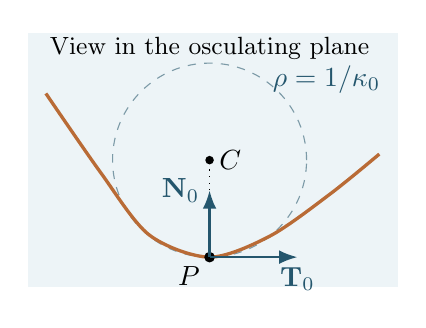
\begin{tikzpicture}[scale=.77,>=Latex]
 \fill[lightblue] (-3,-.5) rectangle (3.1,3.7);
 \draw[inkblue!60,dashed] (0,1.6) circle (1.6);
 \draw[accent,very thick] plot[smooth] coordinates {(-2.7,2.7) (-1.8,1.4) (-1,.37) (0,0) (1,.35) (2,1.05) (2.8,1.7)};
 \fill (0,0) circle(2.5pt) node[below left] {$P$};
 \fill (0,1.6) circle(2pt) node[right] {$C$};
 \draw[->,thick,inkblue] (0,0)--(1.45,0) node[below] {$\T_0$};
 \draw[->,thick,inkblue] (0,0)--(0,1.1) node[left] {$\N_0$};
 \draw[dotted] (0,1.1)--(0,1.6);
 \node[inkblue] at (1.93,2.93) {$\rho=1/\kappa_0$};
 \node[font=\small] at (0,3.45) {View in the osculating plane};
\end{tikzpicture}
\end{center}

\heading{Explore with the rollercoaster cart}
\begin{enumerate}
 \item \textbf{Finish the helix.} Add $\T$, $\N$, and $\B$ successively. Check the right-hand rule. Turn on $a_T\T$ and $a_N\N$, then pause and inspect the two planes and circle.
 \item \textbf{Change the viewpoint.} Compare \emph{World frame} with \emph{Ride with JT}. The camera follows the point in both views; only the second turns with the local frame. Drag to rotate. The displayed derivatives always refer to the original fixed coordinates.
 \item \textbf{Change the motion.} On the changing-speed ellipse or parabolic swoop, find where $a_T$ changes sign. A small circle means large $\kappa$, but large $a_N$ also depends on speed: $a_N=s^2\kappa$.
 \item \textbf{Test the limiting case.} On the straight line, $\kappa=0$. The tangent and normal plane exist, but there is no distinguished $\N$, $\B$, osculating plane, or finite osculating circle. If $s=0$ instead, even $\T=\V/s$ would be undefined.
\end{enumerate}
The arrows use display scales, and finite plane patches represent infinite planes. Playback rate changes how fast the presentation runs; it does not change the functions being differentiated. The track specifies a motion, not a gravity-driven mechanical model.

\newpage
\tagline{REFERENCE FOR THE ROLLERCOASTER MENU}
\heading{Positions and analytic derivatives}
The Lecture 6 helix is worked out above. Each additional track uses the same formulas for $\T,\N,\B,a_T,a_N,\kappa$ and local geometry. All derivatives below are with respect to $t$.

\subhead{Wavy sky ring.}
\begin{align*}
 \R&=\langle2\cos t,\,2\sin t,\,0.6\sin3t\rangle,\\
 \V&=\langle-2\sin t,\,2\cos t,\,1.8\cos3t\rangle,\\
 \A&=\langle-2\cos t,\,-2\sin t,\,-5.4\sin3t\rangle.
\end{align*}
\subhead{Trefoil knot.}
\begin{align*}
 \R&=\langle\sin t+2\sin2t,\,\cos t-2\cos2t,\,-\sin3t\rangle,\\
 \V&=\langle\cos t+4\cos2t,\,-\sin t+4\sin2t,\,-3\cos3t\rangle,\\
 \A&=\langle-\sin t-8\sin2t,\,-\cos t+8\cos2t,\,9\sin3t\rangle.
\end{align*}
\subhead{Ellipse: changing speed.} Set $u=t+0.45\sin t$. Then $u'=1+0.45\cos t>0$, $u''=-0.45\sin t$, and
\begin{align*}
 \R&=\langle3\cos u,\,1.7\sin u,\,0\rangle,\\
 \V&=u'\langle-3\sin u,\,1.7\cos u,\,0\rangle,\\
 \A&=u''\langle-3\sin u,\,1.7\cos u,\,0\rangle
 +(u')^2\langle-3\cos u,\,-1.7\sin u,\,0\rangle.
\end{align*}
This parametrization is chosen for comparison; it is not the Kepler timing of an orbit.

\subhead{Parabolic swoop.}
\[
 \R=\langle t,t^2/2,0\rangle,\quad \V=\langle1,t,0\rangle,
 \quad\A=\langle0,1,0\rangle.
\]
Here $a_T=t/\sqrt{1+t^2}$, $a_N=1/\sqrt{1+t^2}$, and $\kappa=(1+t^2)^{-3/2}$.

\subhead{Expanding corkscrew.} Put $q=0.7+0.1t$. Then
\begin{align*}
 \R&=\langle q\cos t,\,q\sin t,\,0.25t\rangle,\\
 \V&=\langle0.1\cos t-q\sin t,\,0.1\sin t+q\cos t,\,0.25\rangle,\\
 \A&=\langle-0.2\sin t-q\cos t,\,0.2\cos t-q\sin t,\,0\rangle.
\end{align*}
\subhead{Straight-line express.}
\[
 \R=\langle t,0,0\rangle,\quad \V=\T=\langle1,0,0\rangle,
 \quad\A=\mathbf0,\quad a_T=a_N=\kappa=0.
\]
At $t_0$, the normal plane is $x=t_0$. The normal component of acceleration is the zero vector, even though $\N$ itself is undefined.

\newpage
\tagline{NEW TOPIC: KEPLER'S LAWS}
\heading{From an assigned track to a force that determines motion}
In the rollercoaster presentation, we chose $\R(t)$ and differentiated it. For an orbit, we instead specify the force and initial position and velocity, then ask which motion follows. Lecture 6 used this idea for a projectile under constant downward acceleration. Far from Earth's surface, gravitational acceleration must be described by an inverse-square law.

\demolink{https://gtevelev-max.github.io/math233h/solar-system/}{Presentation 2: solar system and Kepler motion}

\heading{The three laws we will introduce and explain}
\begin{enumerate}
 \item \textbf{Ellipse law.} A planet travels on an ellipse with the Sun at one focus.
 \item \textbf{Equal-area law.} The radius vector from the Sun to the planet sweeps equal areas in equal time intervals.
 \item \textbf{Period law.} For bodies orbiting the same Sun, the square of the orbital period is proportional to the cube of the semimajor axis: $P^2\propto a^3$.
\end{enumerate}
These describe planetary motion. In Newton's ideal model, we will first derive the second law, then the first, then the third. We assume a fixed Sun, neglect interactions among orbiting bodies, and consider nonradial bound orbits when discussing ellipses and periods.

\heading{Newton's gravitational law}
Place the Sun, of mass $M$, at the origin. For an orbiting body of mass $m$, write $r=\norm{\R}>0$ and $\mu=GM$. The force and acceleration are
\[
 \boxed{\F=-\frac{GMm}{r^3}\R,\qquad
 \A=\R''=-\frac{\mu}{r^3}\R.}
\]
The force magnitude is $GMm/r^2$; the additional factor $1/r$ converts $\R$ to a unit direction. The minus sign points toward the Sun. The gravitational constant $G$ is different from the approximately constant near-surface acceleration $g$ used for projectiles.

\heading{A conserved vector fixes the orbital plane}
Define \textbf{specific angular momentum} (angular momentum per unit mass) by
\[
 \HH=\R\times\V.
\]
Using the product rule for cross products,
\[
 \HH'=\V\times\V+\R\times\A
 =\mathbf0+\R\times\left(-\frac{\mu}{r^3}\R\right)=\mathbf0.
\]
Thus $\HH$ is constant. If $\HH\ne\mathbf0$, every position and velocity lies in the fixed plane through the Sun perpendicular to $\HH$. This conclusion holds for \emph{any central force}, since all that was needed here was $\A\parallel\R$. The actual angular momentum is $m\HH$.

\subhead{Begin with Earth.} Keep the eight planets visible and Earth in focus. Toggle $\R$, $\V$, $\F$, and $\HH$. Identify the Sun-to-body direction, the tangent, the inward force, and the normal to the orbital plane. Rotate the scene to separate these directions visually.

\newpage
\tagline{KEPLER'S SECOND LAW}
\heading{Equal time, equal swept area}
Let $h=\norm{\HH}>0$, and orient the orbital plane so that polar angle $\theta$ increases in the direction of motion. In polar coordinates,
\[
 \R=r\,\mathbf e_r,\qquad
 \V=r'\,\mathbf e_r+r\theta'\,\mathbf e_\theta,
 \qquad h=r^2\theta'.
\]
An infinitesimal polar sector has area $dA=\tfrac12r^2\,d\theta$. Therefore
\[
 \boxed{\frac{dA}{dt}=\frac12r^2\theta'=\frac h2,\qquad
 A(t_2)-A(t_1)=\frac h2(t_2-t_1).}
\]
Because $h$ is constant, equal time intervals sweep exactly equal areas. The proof uses centrality of the force, not the inverse-square dependence. Inverse-square gravity will be needed for the ellipse law.

\begin{center}
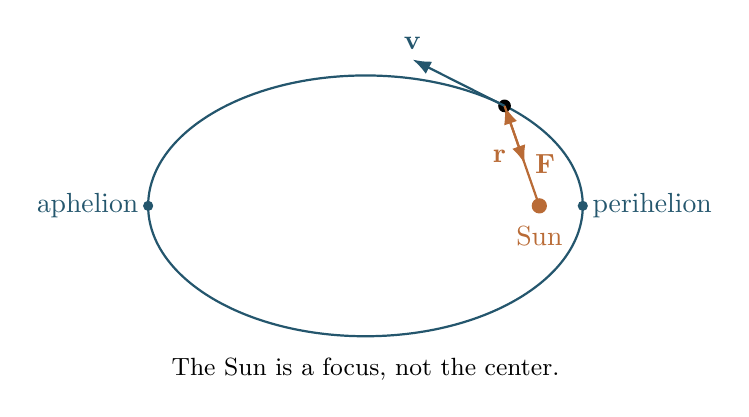
\begin{tikzpicture}[scale=.92,>=Latex]
 \draw[inkblue,thick] (0,0) ellipse (3 and 1.8);
 \fill[accent] (2.4,0) circle (3pt) node[below=4pt] {Sun};
 \fill[inkblue] (-3,0) circle(2pt) node[left] {aphelion};
 \fill[inkblue] (3,0) circle(2pt) node[right] {perihelion};
 \draw[->,accent,thick] (2.4,0)--(1.92,1.38) node[midway,left,xshift=-2pt] {$\R$};
 \fill (1.92,1.38) circle(2.5pt);
 \draw[->,inkblue,thick] (1.92,1.38)--(.65,2.02) node[above] {$\V$};
 \draw[->,accent,thick] (1.92,1.38)--(2.2,.58) node[right] {$\F$};
 \node[font=\small] at (0,-2.25) {The Sun is a focus, not the center.};
\end{tikzpicture}
\end{center}

\subhead{Compare sectors in the presentation.} Enable swept areas. Fix an increment $\Delta t$ for the focused orbit, and compare the complete sectors near perihelion and aphelion. They have equal areas, although their angles and arc lengths differ. At smaller $r$, the angular speed $\theta'=h/r^2$ is larger. Different bodies have different $h$, so equal \emph{absolute} time intervals need not sweep the same area across different orbits.

\heading{Connect this to tangential and normal acceleration}
An inward force is not generally a principal-normal force: ``toward the Sun'' and ``perpendicular to the velocity'' are different directions. For solar gravity,
\[
 a_T=\frac{\V\cdot\A}{s}
 =-\frac{\mu\,\R\cdot\V}{r^3s}
 =-\frac{\mu r'}{r^2s}.
\]
The body slows down while moving outward ($r'>0$), and speeds up while moving inward ($r'<0$). At perihelion and aphelion, $r'=0$, so the acceleration is purely normal. On a circle it is purely normal everywhere.

\subhead{Make the contrast visible.} Earth's orbit is nearly circular. Compare Mercury, then select \emph{Comet (Halley)} to make the change in speed and sector shape much more pronounced. The sector boundary follows the orbital arc; a triangle joining two sampled positions is only an approximation.

\newpage
\tagline{KEPLER'S FIRST LAW: A VECTOR-CALCULUS DERIVATION}
\heading{Why does inverse-square gravity produce a conic?}
We know that $\HH=\R\times\V$ is constant. Define one more vector,
\[
 \EE=\frac{\V\times\HH}{\mu}-\frac{\R}{r}.
\]
It is called the eccentricity vector. We will show that it is constant. First,
\[
 \frac{d}{dt}\left(\frac{\R}{r}\right)
 =\frac\V r-\frac{\R(\R\cdot\V)}{r^3},
 \qquad r'=\frac{\R\cdot\V}{r}.
\]
The vector triple-product identity gives
\begin{align*}
 \A\times\HH
 &=-\frac{\mu}{r^3}\R\times(\R\times\V)\\
 &=-\frac{\mu}{r^3}\bigl[\R(\R\cdot\V)-r^2\V\bigr]
 =\mu\frac{d}{dt}\left(\frac{\R}{r}\right).
\end{align*}
Since $\HH'=\mathbf0$, we obtain $\EE'=\mathbf0$. Let $e=\norm{\EE}$. For $e>0$, choose the positive $x$-axis in the fixed direction of $\EE$, and let $\theta$ be the angle from it to $\R$. Dot the definition of $\EE$ with $\R$:
\[
 er\cos\theta
 =\frac{\R\cdot(\V\times\HH)}\mu-r
 =\frac{\HH\cdot(\R\times\V)}\mu-r
 =\frac{h^2}{\mu}-r.
\]
Writing $p=h^2/\mu$, this is the polar equation
\[
 \boxed{r=\frac{p}{1+e\cos\theta}.}
\]
\heading{For $0\le e<1$, the conic is an ellipse}
If $e>0$, write $x=r\cos\theta$, $y=r\sin\theta$. The relation $r+ex=p$ gives $\sqrt{x^2+y^2}=p-ex$. Squaring and completing the square produces
\[
 \frac{(x+ae)^2}{a^2}+\frac{y^2}{b^2}=1,\qquad
 a=\frac p{1-e^2},\quad b=a\sqrt{1-e^2}.
\]
The center is $(-ae,0)$ and one focus is the Sun at $(0,0)$. The vector $\EE$ points toward perihelion. If $e=0$, the equation is the circle $r=p$, with the Sun at its center.

\subhead{Why the bound-orbit condition matters.} The conserved energy per unit mass is
\[
 \varepsilon=\frac12\norm{\V}^2-\frac\mu r,
 \qquad \varepsilon'=\V\cdot\A+\frac{\mu r'}{r^2}=0.
\]
Expanding $\norm{\EE}^2$, using $\V\perp\HH$ and $\R\cdot(\V\times\HH)=h^2$, yields
\[
 e^2=1+\frac{2\varepsilon h^2}{\mu^2}.
\]
For $h>0$, negative energy gives $e<1$ and an ellipse. Zero and positive energy give a parabola and hyperbola, respectively. Thus inverse-square gravity does not make \emph{every} trajectory an ellipse. The case $h=0$ is radial motion and was excluded.

\newpage
\tagline{KEPLER'S THIRD LAW AND SPEED ALONG AN ORBIT}
\heading{The period follows from area and angular momentum}
For an ellipse, $b=a\sqrt{1-e^2}$ and $p=a(1-e^2)$. The first-law calculation therefore gives
\[
 h^2=\mu p=\mu a(1-e^2)=\frac{\mu b^2}{a}.
\]
The total area of the ellipse is $\pi ab$. The equal-area law says that this is also $(h/2)P$, where $P$ is one orbital period. Consequently
\[
 P=\frac{2\pi ab}{h},\qquad
 P^2=\frac{4\pi^2a^2b^2}{h^2}
 =\boxed{\frac{4\pi^2}{\mu}a^3}.
\]
The eccentricity cancels. Two bound orbits around the same Sun with the same semimajor axis have the same period, even if their shapes are very different. In the fixed-Sun approximation, $\mu=GM$ is the same for all the orbiting bodies. For the exact relative two-body problem, replace it by $G(M+m)$.

\heading{How quickly does the body move?}
Combining $e^2=1+2\varepsilon h^2/\mu^2$ with $h^2=\mu a(1-e^2)$ gives $\varepsilon=-\mu/(2a)$. Substitute this into the energy formula:
\[
 \boxed{s^2=\mu\left(\frac2r-\frac1a\right).}
\]
For a fixed ellipse, the speed is largest at the smallest distance and smallest at the largest distance. At the endpoints of the major axis,
\[
 r_{\rm peri}=a(1-e),\qquad r_{\rm aph}=a(1+e),\qquad
 s_{\rm peri}r_{\rm peri}=s_{\rm aph}r_{\rm aph}=h,
\]
so
\[
 \boxed{\frac{s_{\rm peri}}{s_{\rm aph}}=\frac{1+e}{1-e}.}
\]
This explains why a highly eccentric comet is a useful comparison with Earth: it spends much of its time far from the Sun, then passes rapidly through perihelion.

\heading{Use the solar presentation to distinguish the laws}
\begin{enumerate}
 \item \textbf{First law: shape and focus.} Pause on a more eccentric orbit. Locate the center of the ellipse and the Sun separately. Predict which point is perihelion.
 \item \textbf{Second law: time within one orbit.} Keep the sector duration fixed for the focused body. Compare equal-time regions at different distances, and compare the displayed speed and force magnitudes.
 \item \textbf{Third law: compare whole orbits.} Compare the displayed periods and semimajor axes for different bodies. Doubling $a$ multiplies $P$ by $2^{3/2}$, not by $2$.
 \item \textbf{Return to the moving frame.} At perihelion, identify $\T$ and $\N$ from velocity and acceleration. Away from perihelion or aphelion, explain why the Sun need not lie on the principal-normal line.
\end{enumerate}
\subhead{A useful distinction.} Kepler's second law follows from any central force. The ellipse shape and period relation established here depend on the inverse-square gravitational law.

\newpage
\tagline{HOW THE PRESENTATION PUTS TIME ON AN ELLIPSE}
\heading{The eccentric anomaly and Kepler's equation}
A geometrical ellipse alone does not prescribe a motion. Constant polar angular speed generally violates equal areas. Instead use the eccentric anomaly $E$, with perihelion at $E=0$:
\[
 \R(E)=\langle a(\cos E-e),\ b\sin E,\ 0\rangle,
 \qquad b=a\sqrt{1-e^2}.
\]
The swept area satisfies
\[
 \frac{dA}{dE}
 =\frac12\left(x\frac{dy}{dE}-y\frac{dx}{dE}\right)
 =\frac{ab}{2}(1-e\cos E).
\]
Integrating from perihelion and imposing $dA/dt=h/2$ gives
\[
 E-e\sin E=n(t-\tau),\qquad
 n=\frac h{ab}=\sqrt{\frac\mu{a^3}}=\frac{2\pi}{P},
\]
where $\tau$ is a perihelion time. More generally the right side is $M_0+n(t-t_0)$. This is \textbf{Kepler's equation}; $M$ is called the mean anomaly. Since $1-e\cos E>0$ for $e<1$, time increases with $E$.

Differentiate to obtain the velocity used by the animation:
\[
 \frac{dE}{dt}=\frac{n}{1-e\cos E},\qquad
 \V=\frac{n}{1-e\cos E}\langle-a\sin E,\ b\cos E,\ 0\rangle.
\]
Then $\norm{\R\times\V}=nab=h$. Two unwrapped values $E_1,E_2$ enclose the exact area
\[
 \Delta A=\frac{ab}{2}\bigl[(E_2-e\sin E_2)-(E_1-e\sin E_1)\bigr]
 =\frac h2\,\Delta t.
\]
A fixed spatial rotation places each orbit in its own plane without changing these identities.

\heading{Using and interpreting the solar model}
The presentation starts with all eight planets and the comet enabled, with Earth in focus. Select \emph{Comet (Halley)}, then use \emph{Perihelion} or \emph{Aphelion} to pause at either extreme. Its \emph{Encounter} pace makes the fast passage near the Sun easier to inspect. The default equal-time increment is $P/12$ for the focused body; $P/8$ and $P/24$ are also available.

Each body follows an ideal fixed Kepler orbit, not a current ephemeris; mutual perturbations and comet outgassing are omitted. Halley's adopted orbit has $a\approx17.834$ AU, $e\approx0.96714$, and $P\approx75.31$ years. Its assumed mass, $10^{14}$ kg, is only a teaching value for the force calculation.\footnote{NASA/JPL Solar System Dynamics: \href{https://ssd.jpl.nasa.gov/planets/approx_pos.html}{\emph{Approximate Positions of the Planets}}, Table 1, for planetary J2000 elements (Earth--Moon barycenter for Earth); \href{https://ssd.jpl.nasa.gov/sb/elem_tables.html}{\emph{Small-Body Orbital Elements}}, sample 1P/Halley record, for the comet.} Distances use a linear scale and markers are enlarged. The comet's force and velocity arrows show \emph{directions} at fixed display lengths; read their numerical magnitudes. Its tail is schematic and points away from the Sun. It is not a force vector.

\heading{Questions to close the lecture}
\begin{enumerate}[itemsep=3pt]
 \item Can $\A\ne\mathbf0$ while speed stays constant? Can $\kappa=0$ while speed changes?
 \item Why does a central force conserve $\HH$, and why does that imply equal areas?
 \item Which extra property of gravity makes the bound orbit an ellipse?
 \item How can a comet have a long period while moving very quickly near the Sun?
\end{enumerate}
\end{document}
